\documentclass[12pt, a4paper]{article}

\usepackage[utf8]{inputenc}
\usepackage[T1]{fontenc}
\usepackage[francais]{babel}
%\usepackage{xcolor}
\usepackage{amsmath}
\usepackage{amssymb}
\usepackage{hyperref}

\usepackage{amsthm}  %%%%% ajout 
\newtheorem*{theo}{Théorème} %%%%% ajout

%%%pour inclure des images
\usepackage{graphicx}
%TODO: \graphicspath{ {images/} }


\title{Résolution de l'équation de \textsc{Laplace}, par la méthode de Monte-Carlo}
\author{Victor \textsc{Schneider}, Christophe \textsc{Riviere}, Fabien \textsc{Delhomme}}
\begin{document}
%Définition de commandes
%\newcommand{\impo}[1]{\emph{#1}}
%Fin de définition de commandes
\maketitle
\begin{abstract}
    L'objectif de ce projet est de calculer une solution de l'équation de \textsc{Laplace} à l'aide de la
    méthode de Monte-Carlo pour des domaines réguliers dans $\mathbb{R}^2$. Tout le code de ce
    projet est posté en ligne à cette adresse:
    \url{https://github.com/superLinab/ProjetScientifique}.
\end{abstract}

%TODO: DIRE QUEL EST LE BUT QUE L'ON S'EST FIXÉ DANS CE PROJET
\section{Présentation de la méthode de Monte-Carlo}

\subsection{Introduction}

La méthode de Monte-Carlo est une méthode d'approximation numérique qui s'appuie sur les propriétés
de la marche aléatoire.
\smallbreak
Cette méthode est très utilisée dans les domaines scientifiques nécessitants des approximations
numériques. Un exemple, lors de l'expérience permettant de mettre en évidence les oscillations des
neutrinos (en 2001), il était nécessaire de comparer les données énergétiques expérimentales avec
les valeurs numériques que donnait la théorie, valeurs qu'il a fallu estimer numériquement. On a
utiliser pour ce faire la méthode de Monte-Carlo\footnote{source:
    \url{http://arxiv.org/abs/nucl-ex/0110005v1}}.

\begin{flushleft}
    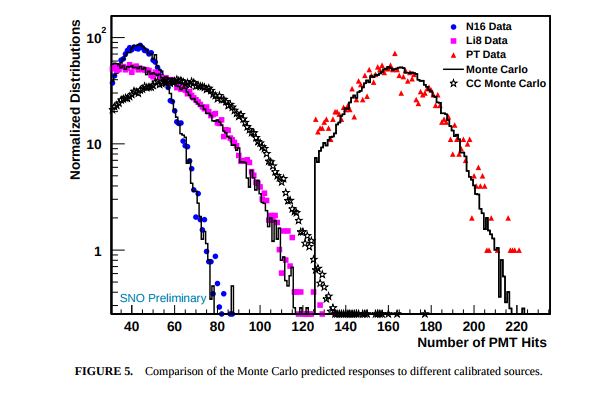
\includegraphics[width=17cm]{exMC}
\end{flushleft}

\subsection{Idée générale de la méthode}

\begin{theo}
    Théorème de transfert dans le cas d'une loi continue.

    Soit $f : \mathbb{R}^n \rightarrow \mathbb{R}$ la fonction densité associée à la variable
    aléatoire $X = (X_1, X_2,...,X_n)$.

    Alors\[ \mathbb{E} \left( \phi(X_1, ..., X_n) \right) =  \int_{\mathbb{R}^n}
    \phi(x_1,...,x_n)f(x_1,...,x_n) \, \mathrm{d}x_1...\mathrm{d}x_n.  \] \end{theo}

Si l'on veut calculer une valeur numérique $A$ bien exprimée, on peut la voir grâce au théorème ci
-dessus comme une espérance.

Soit $A$ notre valeur numérique à calculer sur un pavé, \[ A = \int_{[a,b]^n}
\phi(x_1,...,x_n)f(x_1,...,x_n) \, \mathrm{d}x_1...\mathrm{d}x_n.  \] Alors \[ A = \mathbb{E} \left(
\phi(X_1, ..., X_n) \right).  \] où les $X_i$ sont des variables indépendantes suivant toutes la loi
uniforme sur $[a,b]$.  \medbreak L'idée derrière cette méthode est de pouvoir approximer une valeur
numérique par une moyenne de marches aléatoires. Le théorème clef qui autorise cette démarche est la
loi forte des grands nombres :

\begin{theo} Loi forte des grands nombres.

    Soit $(Y_k)_{k\ge 0}$ une suite de variables aléatoires indépendantes et suivant toutes la même
    loi, à valeurs dans $\mathbb{R}^n$. On suppose $\mathbb{E}(|Y_1|) < +\infty $. Alors

    \[ \frac{Y_1+...+Y_N}{N}\underset{N\to+\infty}{\longrightarrow}\mathbb{E}(Y_1)\; \text{presque
    sûrement.} \] \end{theo}

Autrement dit, si l'on prend un $N$ assez grand, on peut estimer une espérance de manière
relativement précise. On peut alors estimer notre valeur numérique $A$ "simplement" par une moyenne
de variable aléatoire. On peut donc utiliser cette méthode pour effectuer un calcul numérique de
$A$.

\[ A \approx \frac{\phi(Y_1)+...+\phi(Y_N)}{N} \] où tous les $Y_i$ suivent la même loi que $X$
précédemment.

Or numériquement, on sait faire une moyenne, et on sait modéliser des variables aléatoires.

\subsection{Monte-Carlo appliquée à la résolution d'un problème de \text{Laplace}}

\subsubsection{Problème de \textsc{Dirichlet}}

Nous allons utiliser cette méthode pour établir des solutions numériques au problème de \textsc{Dirichlet}
suivant : \medbreak

Soit $\Omega \in \mathbb{R}$ un domaine borné, et $\partial\Omega$ son bord. On cherche $u$ telle
que \[\bigtriangleup u(x) = 0, \quad \forall x \in \Omega\] \[u(x) = g(x), \quad \forall x \in
\partial \Omega, \quad \text{g connue}\]

Rappelons que dans un problème de \textsc{Dirichlet}, il y a existence et unicité de la solution, et que
celle-ci atteint son maximum et son minimum sur le bord du domaine.  \medbreak


Malheureusement, le domaine est mathématiquement continu, ce que l'ordinateur ne peut pas gérer.
Nous allons donc le discrétiser, et nous ramener à \emph{un problème de \textsc{Dirichlet} discret}.
\medbreak

\subsubsection{Problème de \textsc{Dirichlet} discret }

Comment construire ce problème de \textsc{Dirichlet} discret ?

Si l'on considère notre discrétisation de pas $h$. Donc on passe d'une case à l'autre en ajoutant
$h$ à nos abscisses, respectivement ordonnées.

$u$ prend ses valeurs dans $\mathbb{R}^2$, la formule de Taylor nous donne (on travaille sur les
abscisses mais c'est exactement pareil pour les ordonnées) : \[ \begin{cases} u(x+h,y) - u(x,y) &=
        h\partial_1 u(x,y) + \frac{h^2}{2}\partial_1^2 u(x,y)+ O(h^3)\\ u(x-h,y) - u(x,y) &=
        -h\partial_1 u(x,y) + \frac{h^2}{2}\partial_1^2 u(x,y)+ O(h^3)\\ \end{cases} \] En sommant
    les deux on obtient : \[ \partial_1^2 u(x,y)= \frac{1}{h^2}\left[u(x+h,y) + u(x-h,y) - 2u(x,y)
    \right] + O(h) \] $u(x+h, y) $ et $u(x+h, y) $ sont les voisins de $u(x,y)$.  On se rend compte
    qu'on peut alors approximer les dérivées secondes spatial par des différences entres les
    voisins.  \smallbreak

D'où on peut définir le \emph{Laplacien discret} pour toute fontion $F$ de $\Omega \cup \partial
\Omega$ dans $\mathbb{R}$ :

\[ \overline{\bigtriangleup}F = \sum\limits_{\substack{\Omega_d \cup \partial \Omega_d \\ y \sim x}}
(F(y) - F(x)) \] avec $y\sim x$ signifiant que $y$ est voisin de $x$ et $\Omega_d$ le domaine
discrétisé.

Poser cette approximation du Laplacien est pertinent car le calcul effectué avant nous montre
qu'alors

\[ \bigtriangleup F = \frac{1}{h^2}\overline{\bigtriangleup}F + O(h) \] avec $h \sim 0$.

On peut alors approcher le problème de \textsc{Dirichlet} par un problème de \textsc{Dirichlet} discret :
\[\overline{\bigtriangleup} u(x) = 0, \quad \forall x \in \Omega_d\] \[u(x) = g(x), \quad \forall x
\in \partial \Omega_d, \quad \text{g connue}\]

\subsubsection{Résolution du problème de \textsc{Dirichlet} discret} Il s'avère que dans ces conditions, pour
tout point $x$ du domaine discrétisé, on peut atteindre le bord par une marche aléatoire.  En effet,
de la même manière que dans la marche de l'ivrogne, celui-ci est sur de rentrer chez lui après un
déplacement plus ou moins long, notre marche atteindra le bord avec une probabilité de 1.

Quel intérêt y a-t-il a mettre ceci en évidence ?

Et bien cela valide notamment le théorème suivant :

\begin{theo} $\forall x \in \Omega$, la valeur de $u(x)$ est donnée par : \[ u(x) = \sum_{y\in
    \partial A} g(y) P(x, \{y\}) \] avec $P(x, \{y\})$ la probabilité que $y$ soit le premier
    élément de $\partial A$ atteint par la marche aléatoire partant de $x$.  \end{theo}
\emph{Remarque} : D'après ce qui a été dit précédemment $P(x, \{y\})$ est bien une probabilité
puisque $\sum_{y\in \partial A} P(x, \{y\}) = 1$ (on est sûr d'atteindre le bord).  \smallbreak Ce
théorème va alors permettre de coder la méthode de Monte-Carlo, puisque l'on connaît $g(y)$ sur
notre bord discrétisé, et $P(x, \{y\})$ est obtenu grâce à une moyenne de marches aléatoires.

\section{Schéma retenu}

\subsection{Discrétisation}
On commence par discrétiser le domaine choisi. On a choisi de quadriller le domaine.  Au début, nous
avons commencé par utiliser les coordonnées des points du plan puis exécuter la marche aléatoire en
«sautant» de points en points où la distance entre chaque saut est donnée par $1/N$, où $N$ était un
paramètre du schéma.  Malheureusement, au fur et à mesure des pas, à cause des erreurs d'arrondi, on
«sort» de la grille du domaine. Nous avons donc préféré construire une grille (une matrice) qui
représente les points du domaine, puis effectuer la marche aléatoire dans cette grille. Les indices
d'une matrice étant entier, il n'y a plus d'erreur d'arrondi possible.

La discrétisation s'effectue donc grâce à une matrice remplie de $1$ ou $0$ pour indiquer
respectivement si un point se trouve ou non dans le domaine.

\subsection{Marche aléatoire}

Il faut maintenant parcourir tout les points de la grille qui sont à l'intérieure du domaine.
Pour chaque point du domaine, on lance $K$  marches aléatoires qui commencent en ce point. On fait
ensuite la moyenne de toutes les valeurs données par la fonction au bord en tout les points à
l'extérieure du domaine atteints après une marche aléatoire.

\section{Convergence}

\subsection{Mise en oeuvre}
Pour analyser la convergence nous avons utilisés la propriété du schéma d'être stable par «fusion».
C'est-à-dire que si nous avons effectué $K$ marches aléatoires pour chaque point d'un domaine fixé,
nous pouvons raffiner le résultat et lancer $l$ marches aléatoires puis faire la moyenne pondérée entre
les deux résultats pour obtenir une simulation de $K+l$ marches aléatoires (puisque les marches sont
indépendantes les unes des autres).

On utilise donc la formule suivante pour «fusionner» les deux résultats sur un point donnés $(i,j)$
de la grille

\[
    M_{K+l}(i,j) = \frac{ \sum_{i=K}^{i=K+l} v_i + K*M_{K}(i,j) }{ (K + L) }
\]

Où les $v_i$ représentent les nouvelles valeurs trouvées lors du lancement des $l$ marches
aléatoires au point $(i,j)$.

\subsection{Résultats}

Nous avons choisis de faire varier le nombre de marche aléatoire en fixant le maillage de la grille.

En premier lieu, nous exposerons les résultats pour un disque dans $\mathbb{R}^2$.

De plus, nous avons trouvé que le moyen le plus simple de tester cette méthode est tout simplement
d'imposer des conditions linéaires au bord du domaines. En effet, si $g$ est linéaire, alors elle
est elle-même trivialement solution de l'équation de \textsc{Laplace}.

D'où par unicité de la solution au problème de \textsc{Dirichlet}:
\[\forall (x,y) \in \mathcal{D} \quad f(x,y) = g(x,y) \]

Nous avons choisi la norme infinie pour mesurer l'écart entre la solution approchée et la solution
exacte. Pour des raisons purement esthétiques, nous avons fixé dans notre étude $g(x,y) =
-x -y+2$ et nous restreignons tous nos domaines dans le pavé $[0;1]^2$.

Pour la suite nous désignerons $K$ le nombre de marches aléatoires lancées par point, et $N$ le
maillage (d'où $N^2$ le nombre de points de notre grille).

Nous avons mit ce que l'on obtient pour $N = {10, 20, 30}$ et $K = 50$ aux Figure~\ref{image50} et
Figure~\ref{image75}.

\begin{figure}[h!]
    \begin{center}
        \caption{Représentation de la solution approchée pour N = 10, puis N = 20 et N = 30, pour K = 50}
        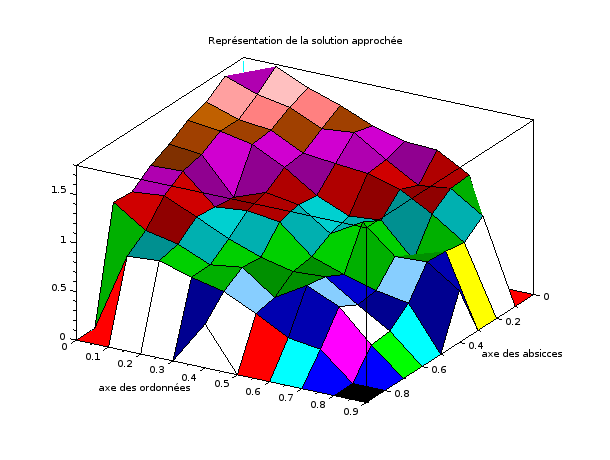
\includegraphics[width=13cm,height=7cm]{ResultatsConvergences/ImageK5S10N10.png}
        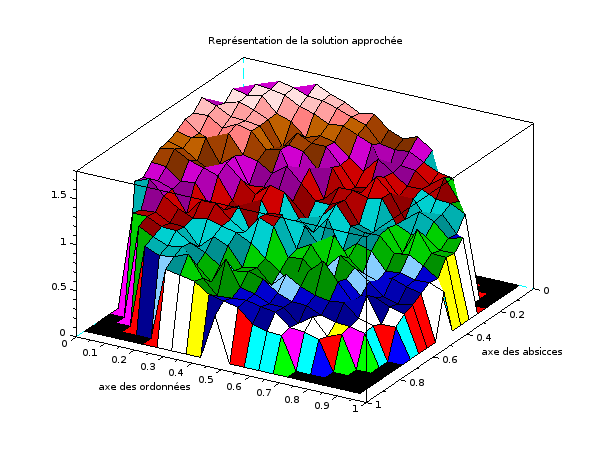
\includegraphics[width=13cm,height=7cm]{ResultatsConvergences/ImageK5S10N20.png}
        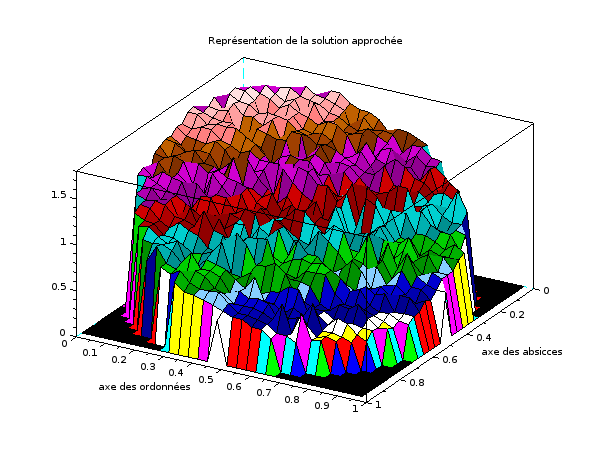
\includegraphics[width=13cm,height=7cm]{ResultatsConvergences/ImageK5S10N30.png}
        \label{image50}
    \end{center}
\end{figure}

\begin{figure}[p]
    \begin{center}
        \caption{Représentation de la solution approchée pour N = 10, puis N = 20 et N = 30, pour K
        = 75}
        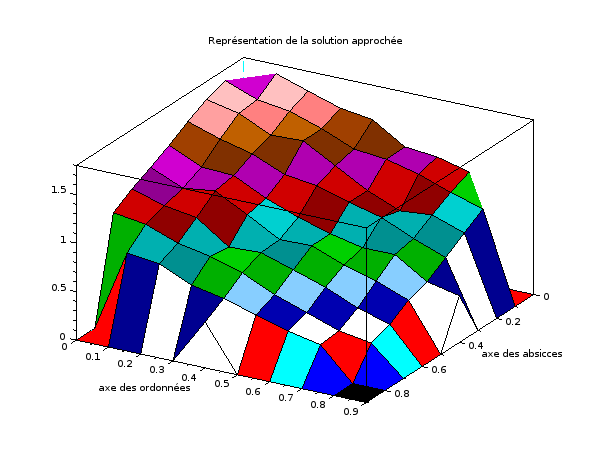
\includegraphics[width=13cm,height=7cm]{ResultatsConvergences/ImageK5S25N10.png}
        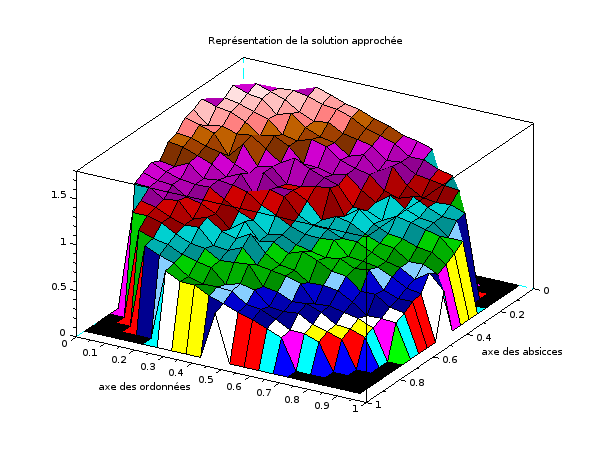
\includegraphics[width=13cm,height=7cm]{ResultatsConvergences/ImageK5S25N20.png}
        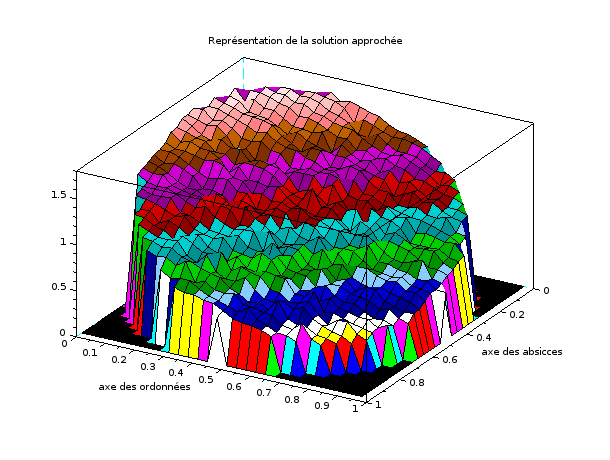
\includegraphics[width=13cm,height=7cm]{ResultatsConvergences/ImageK5S25N30.png}
        \label{image75}
    \end{center}
\end{figure}

Dans le but de déterminer la convergence de notre schéma par rapport au nombre de marche aléatoire
effectuée, nous avons calculé la distance (en norme infinie ) entre notre solution approchée et notre
solution exacte, en fonction du nombre de marche aléatoire lancée. Le résultat est la
Figure~\ref{convergence50} et Figure~\ref{convergence75}.

\begin{figure}[p]
    \begin{center}
        \caption{Représentation de la solution approchée pour N = 10, puis N = 20 et N = 30, pour K = 50}
        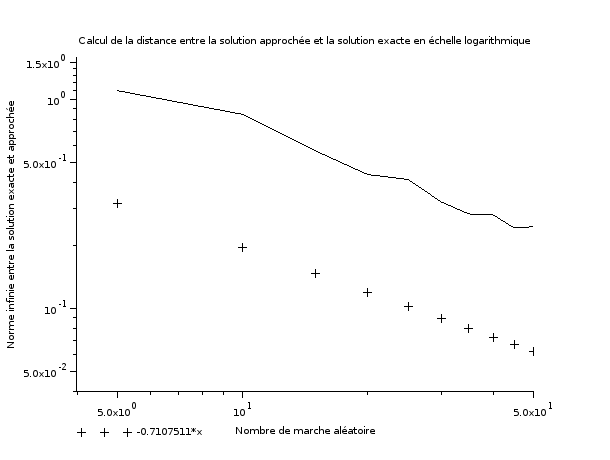
\includegraphics[width=13cm,height=7cm]{ResultatsConvergences/Convergence_K5_S10_N10.png}
        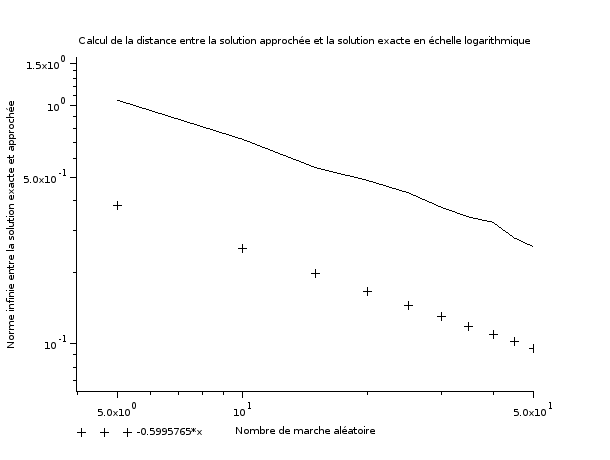
\includegraphics[width=13cm,height=7cm]{ResultatsConvergences/Convergence_K5_S10_N20.png}
        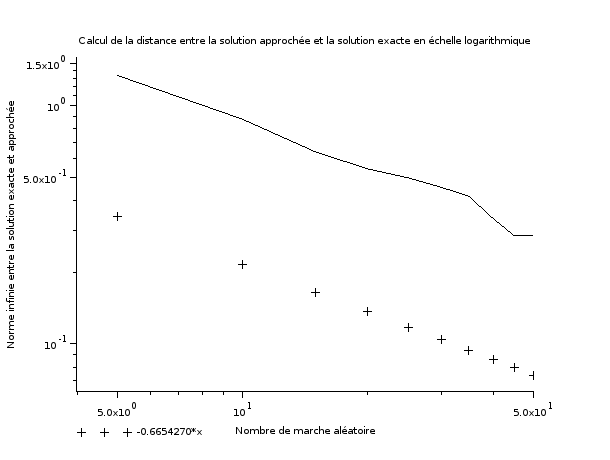
\includegraphics[width=13cm,height=7cm]{ResultatsConvergences/Convergence_K5_S10_N30.png}
        \label{convergence50}
    \end{center}
\end{figure}

\begin{figure}[p]
    \begin{center}
        \caption{Représentation de la solution approchée pour N = 10, puis N = 20 et N = 30, pour K = 75}
        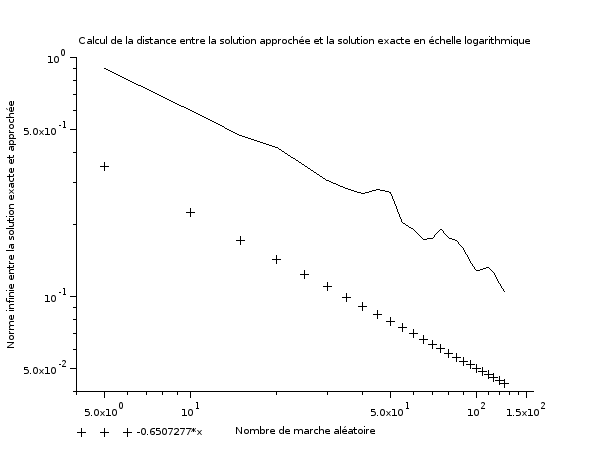
\includegraphics[width=13cm,height=7cm]{ResultatsConvergences/Convergence_K5_S25_N10.png}
        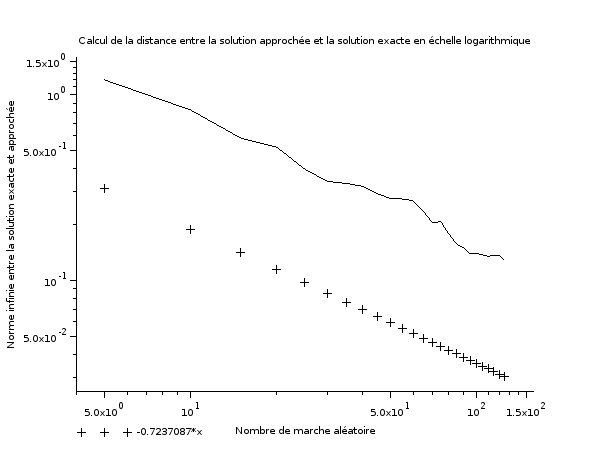
\includegraphics[width=13cm,height=7cm]{ResultatsConvergences/Convergence_K5_S25_N20.png}
        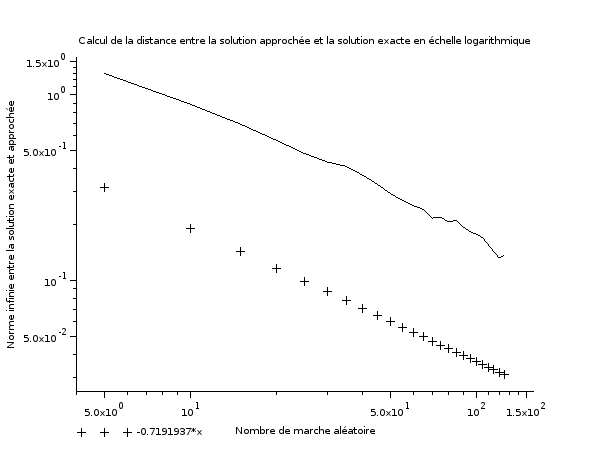
\includegraphics[width=13cm,height=7cm]{ResultatsConvergences/Convergence_K5_S25_N30.png}
        \label{convergence75}
    \end{center}
\end{figure}

Nous avons fait en sorte que les Figure~\ref{convergence50} et Figure~\ref{convergence75} montre la
convergence de notre schéma et que le résultat final soit mointré dans les Figure~\ref{image50} et
Figure~\ref{image75}.
Nous obtenons donc une moyenne de convergence de l'ordre d'environ $O(\frac{1}{K^{0.67}})$.
\section{Avantages et désavantages de la méthode de Monte-Carlo}

On voit tout de suite les intérêts de cette méthode pour le calcul de la solution de l'équation de
\textsc{Laplace}:
\begin{itemize}
	\item La relative simplicité du schéma: la seule difficulté qui s'est présentée fut de créer
		une grille pour lancer la marche aléatoire.
	\item Une parallélisation du calcul possible: la solution est construite point par point
		(!). En effet, contrairement aux schémas classiques qui calculent la valeur en
		chaque point en faisant la moyenne des points autour, ce schéma aléatoire peut par
		exemple calculer la solution en un point précis. On remarque aussi que l'on peut
		facilement stopper le calcul d'une solution pour le reprendre plus tard: il suffit
		de faire une moyenne des deux résultats.
\end{itemize}

Ces avantages s'accompagnent de désavantages certains:
\begin{itemize}
	\item Le bon fonctionnement de l'algorithme dépend en pratique d'un bon générateur de
		hasard. Ce sujet dépasse (de loin) le cadre de ce projet, mais il serait bon de
		vérifier la qualité du hasard proposée par \emph{Scilab}
	\item La difficulté théorique pour justifier la convergence du schéma: il nous faut en effet
		les résultats issue de la théorie de la probabilité, et en particulier de la marche
		aléatoire.
    \item Le temps de calcul est très long ! Nous avons mis plus d'une minute pour générer la
        troisième image de la Figure~\ref{image75}, alors que notre solution approchée est loin de
        notre résultat: la convergence trouvée en une puissance $-0.67$ est très faible.
\end{itemize}

\section{Conclusion}

Cette étude nous aura permis de découvrir une nouvelle méthode radicalement différentes des méthodes
vues en cours puisqu'elle est basée sur un processus aléatoire pour calculer la solution au problème
de \textsc{Dirichlet} (ici, associé à l'équation de \textsc{Laplace}). On a vu que cette méthode était flexible car elle se code
rapidement en \emph{Scilab}, et qu'elle permet de calculer la solution point par point. Mais ces
avantages ont un prix: l'ordre de convergence du schéma est très faible. De plus, il n'est pas
évident de voir comment améliorer cette convergence (alors qu'avec des méthodes plus classiques on
peut essayer de pousser le développement de Taylor un ordre au dessus pour espérer avoir un meilleur
ordre de convergence.)

\end{document}
